% !Mode:: "TeX:UTF-8"

\chapter[绪论]{绪论}[Introduction]

\section{课题背景及意义}[Background and Significance]

\subsection{课题背景}[Background]

% 先写语义分析

% 树结构在语义表示方面的不足, 中英文都出现了语义图标注 (举例)

% 图分析的难点

让机器理解自然语言,是自然语言处理领域最根本也是最重要的问题之一。
要实现在语义层面上理解自然语言,自然语言处理领域的传统方法一般对文本进行自底向上的分词、词性标注、命名实体识别、句法分析,最后才能进行语义分析。
然而,由于中文严重缺乏形态变化,词类与句法成分没有严格的对应关系,导致中文句法分析的精度始终不高。
例如,在英文宾州句法树库(Penn Treebank, PTB)\cite{marcus-etal-1993-building}上目前句法分析准确率已经能达到95\%,而在中文宾州句法树库(Penn Chinese Treebank, CTB)\cite{xue-etal-2005-penn}上则只能达到88\% \cite{dozat-etal-2017-deep}。
为了解决这些问题,哈工大社会计算与信息检索研究中心结合中文重意合、在形式分析上有劣势的语言特点,于2011年在世界上最早提出了跨越句法分析直接进行语义依存分析的思路,并与北京语言大学邵艳秋教授合作标注了中文语义依存树语料库,用树结构融合依存结构和语义关系。

与句法结构相比,句子中词之间的语义关系往往更加复杂。
而传统句法分析中使用的树结构已经无法胜任对如此复杂的语义关系的刻画。
因此,研究者将目光聚集到约束更少的图结构上,希望用图结构来表示这些语义关系。
在英文上,Oepen等人在宾州句法树库的华尔街日报(Wall Street Journal,简称为WSJ)语料上,构建了三种不同标注规范的语义依存图,并于国际语义评测大赛SemEval 2014\cite{oepen-etal-2014-semeval}和SemEval 2015\cite{oepen-etal-2015-semeval}上组织了公开评测任务。
在中文上,哈工大社会计算与信息检索研究中心将中文语义依存树结构扩展为语义依存图,从而更全面地刻画句中词之间的语义关系,并在国际语义评测大赛SemEval 2016\cite{che-etal-2016-semeval}上组织了公开评测任务。
这些语义依存图语料库的构建,吸引了越来越多的研究者在语义依存分析领域开展研究,有力推动了该领域的发展。

与分词、词性标注、句法分析等历史悠久的研究课题相比,语义依存图分析算得上是一个新兴课题,无论是其基础分析方法,还是在不同情境下的应用,以至于如何利用它帮助其他自然语言处理任务,都有待深入探究。
以下从语义依存图分析方法、非规范文本上和多语言文本上的语义依存图分析以及利用语义依存图帮助其他自然语言处理任务四个方面简要阐述相应的研究背景。

1. 语义依存图分析方法。
语义依存图分析器的设计,是该领域最基本也是最重要的问题。
得益于语义依存图与传统句法依存树的相似性,依存图的分析方法可以从大量的依存句法分析任务中借鉴经验。
但图结构在带来更全面的语义表示的同时,也给语义依存分析任务带来了巨大的挑战。
对于依存树结构,每个词只有一个父节点,而在依存图中,每个词可能有多个父节点,这给分析系统带来了很大的不确定性,从而增加了语义依存分析任务的难度。
这也是依存图分析器的设计中亟需解决的研究课题。

2. 非规范文本上的语义依存图分析。
近期有研究表明,基于神经网络的模型尽管在情感分析\cite{zhang-etal-2019-generating}和文本蕴涵\cite{jin-etal-2020-isbert}等自然语言处理任务的标准数据集上取得了很高的精度,但在非规范文本上这些模型的性能会大大下降。
这一发现揭示了目前广泛应用的神经网络模型的脆弱之处,也加强了研究者们对模型鲁棒性的重视。
然而目前这类鲁棒性研究多集中于句子级分类任务上,神经网络模型在语义依存分析等结构化预测任务上的鲁棒性有待深入探究。

3. 多语言文本上的语义依存图分析。
目前语义依存图分析的研究基本都集中在以中英文为代表的少数几种资源丰富的语言上,这是由于人工标注的语义依存图语料只存在于这几种语言上。
然而,对于世界上的大部分语言来说,语义依存图语料难以获取,且人工标注代价较高。
因此,如何充分利用现有人工标注的语料资源,以最小的代价实现对资源稀缺语言的语义依存图分析,也是研究者一直关注的问题。

4. 利用语义依存图帮助其他任务。
语义依存图分析任务最重要的作用之一是为其他自然语言处理任务提供所需的语义信息。
然而,目前大多数该领域的研究仍集中在依存分析器的构建上。
此外,随着基于自注意力网络的上下文相关模型(Bidirectional Encoder Representations from Transformers,简称BERT)\cite{devlin-etal-2018-bert}等预训练模型在自然语言处理各个任务上取得令人瞩目的成绩,句法依存树和语义依存图等人工定义的结构的必要性正面临质疑。
因此,在预训练语言模型大行其道的背景下,如何利用语义依存图帮助其他自然语言处理任务,也是一个重要的研究课题。


\subsection{课题意义}[Significance]

语义依存分析建立在依存理论基础上,是对语义的深层分析,具有形式简洁,易于理解和运用的优势。
其具体可分为两个阶段,首先是根据依存语法建立依存结构,即找出句子中的所有修饰词与核心词对,然后再对所有的修饰词与核心词对指定语义关系。
因此,语义依存分析可以同时描述句子的结构和语义信息。
与传统句法分析相比,语义依存图分析主要有以下三个优点。


\begin{figure}[htpb]
	\begin{center}
			\begin{dependency}[arc edge, arc angle=80, text only label, label style={above}]
				\begin{deptext} [row sep=0.6cm, column sep=.5cm]
					\ ROOT$_0$ \& 早起 $_1$ \& 使$_2$ \& 人$_3$ \&  健康$_4$ \\
				\end{deptext}
				\depedge{1}{3}{\color{black}Root}
				\depedge{3}{2}{\color{black}Exp}
				\depedge{3}{4}{\color{black}Datv}
				\depedge{3}{5}{\color{black}eResu}
				\depedge{5}{4}{\color{black}Exp}
				
				\depedge[edge below]{1}{3}{\color{black}root}
				\depedge[edge below]{3}{2}{\color{black}nsub}
				\depedge[edge below]{3}{4}{\color{black}dobj}
				\depedge[edge below]{3}{5}{\color{black}dep}
			\end{dependency}
			%\caption{语义依存图(上方)与句法依存树(下方)对比示例}
			\bicaption[fig:sdg0]{}{语义依存图(上方)与句法依存树(下方)对比示例}{Fig.$\!$}{Example of semantic dependency graph (upper) and syntactic dependency tree (lower)}
	\end{center}
\end{figure}


首先,它不受到句法分析中树结构的限制,因此可以更全面地覆盖句中各个词之间的语义关系。
图~\ref{fig:sdg0}给出了一个中文语义依存图和句法依存树对比的例子,在句子“早起使人健康”中,“人”同时作为“使”的与事者(Dative, Datv)和“健康”的当事者(Experiencer, Exp),这种关系在有树结构限制的句法标注中难以直接体现,但在语义依存图中则可以直接刻画出来。

其次,语义依存关系比句法依存关系更细化。
例如,“他吃苹果”和“他很高”中的“他”在句法依存分析中都是主语,但前一个句子中的谓词是他的动作,而后一个句子中的谓词描述的是他的特点,这二者的语义是有明显区别的。
因此在语义依存图中前一个“他”标注为施事者(Agent,Agt),后一个“他”标注为当事者(Experiencer,Exp)。
此外,句法依存关系中对句中多个谓词之间的关系没有明确划分。
而在语义依存关系中,定义了并列、条件、转折等详细的谓词间关系。

\begin{figure}[htb]
	\begin{center}
			\begin{dependency}[arc edge, arc angle=80, text only label, label style={above}]
				\begin{deptext} [row sep=0.4cm, column sep=.1cm]
					\ ROOT$_0$ \& 张三 $_1$ \& 昨天$_2$ \& 告诉$_3$ \&  李四$_4$  \& 一件$_5$ \& 事$_6$ \\
				\end{deptext}
				\depedge{1}{4}{\color{black}Root}
				\depedge{4}{2}{\color{black}Agt}
				\depedge{4}{3}{\color{black}Time}
				\depedge{4}{5}{\color{black}Datv}
				\depedge{4}{7}{\color{black}Cont}
				\depedge{7}{6}{\color{black}Quan}
			\end{dependency}
			\bicaption[fig:sdp0]{}{语义依存图示例}{Fig.$\!$}{Example of semantic dependency graph}
	\end{center}
\end{figure}

\begin{figure}[htb]
	\begin{center}
			\begin{dependency}[arc edge, arc angle=80, text only label, label style={above}]
				\begin{deptext} [row sep=0.4cm, column sep=.1cm]
					\ ROOT$_0$ \& 昨天$_1$ \& ,$_2$ \& 张三$_3$ \&  将$_4$  \& 一件$_5$ \& 事$_6$ \& 告诉$_7$ \& 李四$_8$  \\
				\end{deptext}
				\depedge{1}{8}{\color{black}Root}
				\depedge{2}{3}{\color{black}mPunc}
				\depedge{7}{5}{\color{black}mPrep}
				\depedge{7}{6}{\color{black}Quan}
				\depedge{8}{2}{\color{black}Time}
				\depedge{8}{4}{\color{black}Agt}
				\depedge{8}{7}{\color{black}Cont}
				\depedge{8}{9}{\color{black}Datv}
			\end{dependency}
			\bicaption[fig:sdp1]{}{语义依存图示例}{Fig.$\!$}{Example of semantic dependency graph}
	\end{center}
\end{figure}


最后,语义分析可以跨越句子的表层结构直接获取深层语义表达的本质,它通过在句子结构中分析实词间的语义关系来直接回答句子中“谁在何时何地对谁做了什么”等问题。
以图~\ref{fig:sdp0}中的中文句子“张三昨天告诉李四一件事”为例,通过语义依存分析,我们能获知“谁告诉李四一件事?”、“张三告诉谁一件事?”、“张三何时告诉李四一件事?”及“张三告诉李四什么?”等问题的答案。
另外,图~\ref{fig:sdp1}中的句子“昨天,张三将一个秘密告诉李四。”虽然与图~\ref{fig:sdp0}中的句子“昨天,张三将一件事告诉李四”表述形式不同,但含义相同,因此它们的语义依存结构相同。
因此语义依存分析能为问答系统、信息抽取、信息检索等对语义信息要求较高的任务提供很大帮助。
%因此语义依存分析可以解决问答系统、信息抽取、信息检索等任务中的“多句一意”情况。

总的来说,语义依存图分析打破了传统句法依存分析中的树结构,能更全面、直接地获取深层语义表示,提供了更加细粒度的语义关系,从而为需求语义信息的其他自然语言处理任务提供帮助。
从上述研究意义出发,本文围绕中文语义依存图分析任务,立足依存分析技术本身,深入探究在非规范文本和多语言文本上的语义依存图分析,最终利用语义依存图帮助其他自然语言处理任务,为语义依存图的应用提供了一种可能性。

\section{研究现状与分析}[Related Work]

\subsection{句法依存分析}[Syntactic Dependency Parsing]

\subsection{语义依存图分析}[Semantic Dependency Graph Parsing]

\subsection{神经网络模型的鲁棒性}[Robustness of Neural Models]

\subsection{跨语言依存分析}[Cross-Lingual Dependency Parsing]

\subsection{结构化信息在神经网络模型中的应用}[Application of Structural Information in Neural Models]


\section{本文的研究内容及章节安排}[Contents and Chapter Arrangement of the Thesis]

本文围绕中文语义依存图分析开展一系列研究工作。
从语义依存图分析方法本身入手,系统深入地探究了非规范文本和多语言文本上的语义依存图分析,并最终利用语义依存图有效帮助了其他自然语言处理任务。
在这几项研究内容中,语义依存图分析方法是首先需要解决的问题,也是支撑其他任务的基石。
在此基础上,我们探究了在不同场景下的语义依存图分析。
最后,我们研究了利用语义依存图帮助其他自然语言处理任务的方法。

\begin{figure}[htbp]
    \centering
    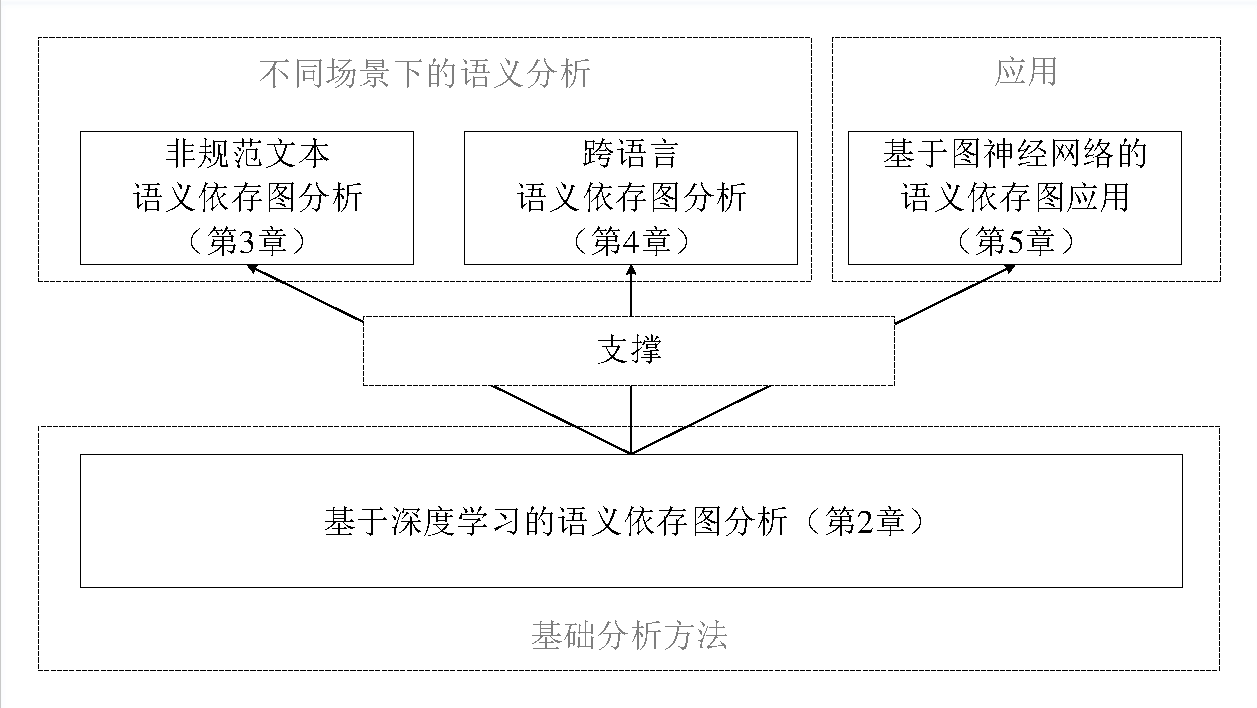
\includegraphics[width=0.95\textwidth]{figures/section_relation.pdf}
    %\caption{论文总体框架}[Structure of the thesis]
    \bicaption[fig:section-relation]{}{论文总体框架}{Fig.$\!$}{Structure of the thesis}
    \label{}
\end{figure}

论文结构框架如图\ref{fig:section-relation}所示,具体来说,本文共包含5章,各章内容组织如下:

在第1章中,本文介绍了中文语义依存图分析的研究背景与意义,并对语义依存图分析的研究现状进行了概述与分析,最后对本文主要内容进行了规划。

在第2章中,针对图结构依存分析的挑战,本文使用基于转移的分析方法,设计了一套用于生成依存图的转移系统,并使用基于栈-长短时记忆网络的模型根据当前转移状态预测下一个转移动作。实验结果表明,本文提出的语义依存图分析方法相比此前的方法取得了显著的性能提升。

在第3章中,针对语义依存图分析在非规范文本上性能远低于规范文本的问题,本文首先设计了一套针对语义依存图分析的对抗样本攻击框架,用于生成使目标语义依存图分析器性能下降的非规范文本。
接着,本文深入探究了对此类非规范文本特征和不同类型分析器的鲁棒性,并在此基础上分别提出了基于对抗样本训练和基于模型融合的方法用于提升现有的依存图分析器的鲁棒性。
实验结果表明,本文提出的对抗样本攻击框架能生成高质量的非规范文本,在它们的帮助下本文有效提升了现有的基于神经网络的依存图分析器的鲁棒性。

在第4章中,针对目前世界上大部分语言上语义依存图语料稀缺,语义依存图分析困难的问题,本文首先对中文语义依存图标注规范进行修改,使其适应多语言场景。
接着,本文提出基于标签转换和图神经网络的方法,首先利用标签转换将现有的多语言大规模通用句法依存语料转换为语义依存图的伪数据,然后使用这些数据和小规模人工标注的语义依存图训练基于图神经网络的编码-解码模型,实现将句法依存语料自动转化为语义依存图语料。
最后,本文使用这些自动转化的语义依存图语料训练跨语言的语义依存图分析器。
实验结果表明,本文提出的跨语言语义依存图分析方法相比于普通的只使用跨语言词向量的方法取得了显著的性能提升。

在第5章中,针对语义依存图分析的应用问题,结合中文的词具有字级别的内部结构的特点,本文提出了基于字级别图结构神经网络编码器,将中文语义依存图融合到预训练模型中,从而增强其表示能力。
本文接着使用这种增强的预训练模型获取的词表示作为其他自然语言处理任务的输入,从而提升其性能。
实验结果表明,本文提出的方法显著提升了语义角色标注和关系抽取任务的性能。

% Local Variables:
% TeX-master: "../thesis"
% TeX-engine: xetex
% End: